\documentclass[preprint,12pt,aps,pra,showkeys,amsmath,amssymb,superscriptaddress,floatfix]{revtex4-2}
\usepackage[T1]{fontenc}
\usepackage[utf8]{inputenc}
\usepackage{amsmath,amssymb,amsthm,mathtools,mathrsfs}
\usepackage{microtype,booktabs,enumitem}
\usepackage{xcolor,tikz,etoolbox}
\usepackage[skins,breakable]{tcolorbox}
\usepackage{needspace}
% Keep diagram geometry independent of REVTeX preprint body spacing.
\AtBeginEnvironment{tikzpicture}{\linespread{1}\selectfont}
\usetikzlibrary{arrows.meta,positioning,calc,fit,decorations.pathreplacing}
\usepackage{graphicx}
\usepackage{hyperref}

\definecolor{MMBlue}{RGB}{0,82,155}
\definecolor{MMOrange}{RGB}{200,80,0}
\tikzset{
 mmnode/.style={draw=MMBlue,rounded corners=2pt,fill=MMBlue!4,align=left,execute at begin node={\raggedright},text width=5cm,font=\fontsize{10}{12}\selectfont,inner sep=6pt},
 mmimport/.style={mmnode,draw=black!65,fill=black!4},
 mmcandidate/.style={mmnode,draw=MMOrange,dashed,fill=MMOrange!5},
 mmrejected/.style={mmnode,draw=black,densely dotted,fill=black!8},
 mmproof/.style={->,thick,MMBlue},
 mmflow/.style={->,semithick,black!70},
 mmrepair/.style={->,dashed,thick,MMOrange},
 mmcandidatearrow/.style={->,dashed,semithick,MMOrange},
 mmnote/.style={font=\scriptsize,fill=white,inner sep=2pt,align=center}}

\usepackage[section]{placeins}
\setlength{\emergencystretch}{3em}
\setlist{itemsep=3pt,topsep=4pt}
\newtheorem{theorem}{Theorem}[section]
\newtheorem{proposition}[theorem]{Proposition}
\newtheorem{lemma}[theorem]{Lemma}
\newtheorem{corollary}[theorem]{Corollary}
\theoremstyle{definition}
\newtheorem{definition}[theorem]{Definition}
\newtheorem{example}[theorem]{Example}
\theoremstyle{remark}
\newtheorem{remark}[theorem]{Remark}
% Avoid isolated statement headings and single-line paragraph fragments.
\BeforeBeginEnvironment{theorem}{\Needspace{6\baselineskip}}
\BeforeBeginEnvironment{definition}{\Needspace{5\baselineskip}}
\BeforeBeginEnvironment{proposition}{\Needspace{5\baselineskip}}
\BeforeBeginEnvironment{lemma}{\Needspace{5\baselineskip}}
\BeforeBeginEnvironment{corollary}{\Needspace{5\baselineskip}}
\clubpenalty=5000
\widowpenalty=5000
\newcommand{\R}{\mathbb R}\newcommand{\Z}{\mathbb Z}\newcommand{\N}{\mathbb N}
\newcommand{\Pa}{\operatorname{Pa}}\newcommand{\Desc}{\operatorname{Desc}}
\newcommand{\cl}{\operatorname{cl}}\newcommand{\cost}{\operatorname{cost}}
\newcommand{\status}{\operatorname{status}}
% Faculty cards: a visual rail groups the five faculties within one agent.
% The rail has no arrowhead and does not represent a proof dependency.
\newcommand{\mmfacultybadge}[1]{%
 \node[circle,draw=MMBlue,line width=1pt,fill=white,
 minimum size=7mm,inner sep=0pt,font=\sffamily\small\bfseries,text=MMBlue]
 at ([xshift=15pt,yshift=-15pt]frame.north west) {#1};}
\newcommand{\mmfacultyrail}{%
 \draw[MMBlue!80,line width=1pt]
 ([xshift=15pt,yshift=2pt]frame.north west)--
 ([xshift=15pt,yshift=-2pt]frame.south west);}
\newtcolorbox{mmfacultybox}[2]{enhanced,breakable,
 colback=MMBlue!4,colframe=MMBlue!4,boxrule=0pt,arc=3pt,
 left=39pt,right=9pt,top=4pt,bottom=4pt,
 before skip=2pt,after skip=2pt,
 fontupper=\small\linespread{1.1}\selectfont,
 overlay unbroken={\mmfacultyrail\mmfacultybadge{#1}},
 overlay first={\mmfacultyrail\mmfacultybadge{#1}},
 overlay middle={\mmfacultyrail},overlay last={\mmfacultyrail}}
\newcommand{\mmfaculty}[3]{%
 \begin{mmfacultybox}{#1}{#2}
 {\sffamily\bfseries\color{MMBlue}#2}\par\smallskip #3
 \end{mmfacultybox}}
\newcommand{\agent}[9]{%
 \Needspace{8\baselineskip}
 \subsubsection{#1}
 \noindent\textbf{Object.} #2\par
 \noindent\textbf{Role.} #3\par\smallskip
 \mmfaculty{E}{Ego}{#4}
 \mmfaculty{M}{Memory}{#5}
 \mmfaculty{I}{Intellect}{#6}
 \mmfaculty{S}{Sense}{#7}
 \mmfaculty{A}{Action}{#8}
 \smallskip\noindent #9\par}

\usepackage{longtable,array,calc}
\providecommand{\tightlist}{\setlength{\itemsep}{2pt}\setlength{\parskip}{0pt}}
\makeatletter
\def\frontmatter@abstract@produce{\par\addvspace{\frontmatter@preabstractspace}%
\begingroup\prep@absbox\unvbox\absbox\post@absbox\endgroup
\addvspace{\frontmatter@postabstractspace}}
\makeatother
\newcommand{\field}[2]{\par\smallskip\noindent\textbf{#1.} #2\par}
\setlength{\emergencystretch}{5em}
\AtBeginEnvironment{verbatim}{\small\linespread{1.0}\selectfont}


\hypersetup{colorlinks=true,linkcolor=MMBlue,urlcolor=MMBlue,pdfauthor={Dibakar Sigdel}}

\begin{document}

\title{Jordan Canonical Form\\[4pt]\large An End-to-End Meta-Math Walkthrough}

\author{Dibakar Sigdel}

\affiliation{Mindverse Computing LLC, Lynnwood, WA 98087, USA}

\date{October 2026}

\begin{abstract}

A complete authored walkthrough of jordan canonical form, with explicit
mathematical contracts, local verification gates, and reusable exports.
The report presents the target theorem, declared imports, a dependency
graph, five-faculty node contracts, a continuous proof, a worked
example, and a hypothesis-repair audit. It is an authored mathematical
exposition, not a deployed-agent transcript or a formal proof-assistant
certificate.

\end{abstract}\maketitle\linespread{1.12}\selectfont

\noindent\textbf{LA-05 / Linear Algebra / Report v1}

\section{Target and import contract}

\begin{theorem}

For every complex square matrix \(A\), prove \(A=PJP^{-1}\) for a
block-diagonal Jordan matrix \(J\), and prove its Jordan blocks are
unique up to permutation.

\end{theorem}

\subsection{Foundations and permitted imports}

Work over C. Import characteristic-polynomial splitting (from the
fundamental theorem of algebra), Cayley--Hamilton \(\chi _A(A)=0\), and
polynomial Bézout for coprime polynomials. Define
\(K_j=\operatorname{ker} N^j\) for a nilpotent restriction. The primary
decomposition and nilpotent-chain basis are constructed below, so they
are not hidden imports.

For each nonzero primary summand let \(s\) be the nilpotency index, set
\(K_0=0\), and set \(K_{s+1}=K_s=V_\lambda\). Finite-dimensional basis
extension and rank--nullity (LA-01) justify complement choices and
dimension counts.

\clearpage\section{Node interaction workflow}

\begin{center}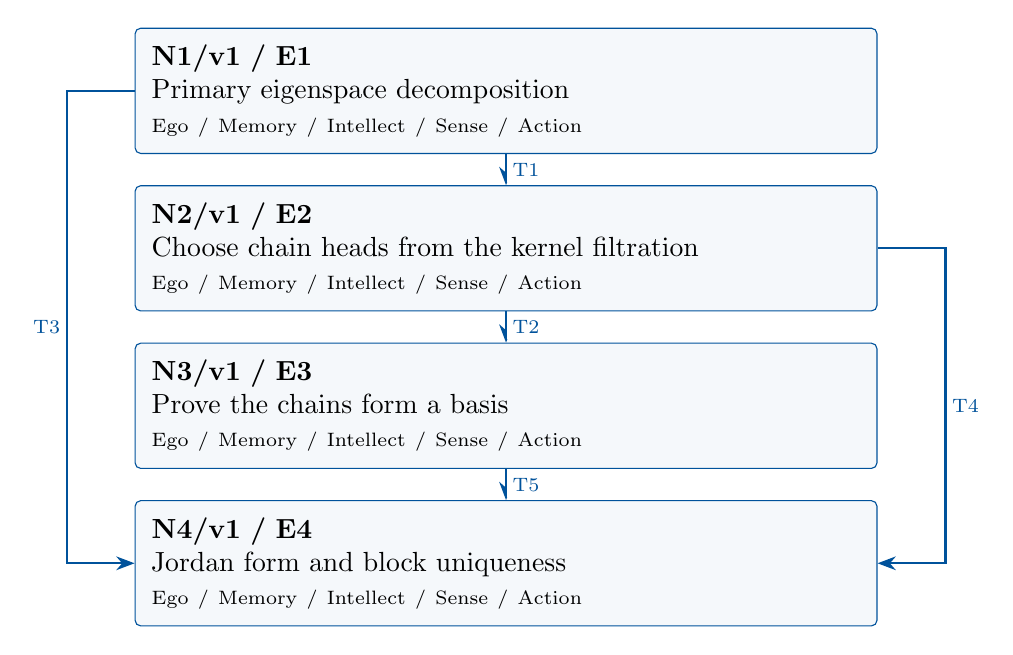
\begin{tikzpicture}[>=Stealth,x=1cm,y=1cm]

\node[mmnode,text width=9cm,minimum height=1.25cm] (N1) at (0,0.0) {\textbf{N1/v1 / E1}\\Primary eigenspace decomposition\\{\scriptsize Ego / Memory / Intellect / Sense / Action}};

\node[mmnode,text width=9cm,minimum height=1.25cm] (N2) at (0,-2.0) {\textbf{N2/v1 / E2}\\Choose chain heads from the kernel filtration\\{\scriptsize Ego / Memory / Intellect / Sense / Action}};

\node[mmnode,text width=9cm,minimum height=1.25cm] (N3) at (0,-4.0) {\textbf{N3/v1 / E3}\\Prove the chains form a basis\\{\scriptsize Ego / Memory / Intellect / Sense / Action}};

\node[mmnode,text width=9cm,minimum height=1.25cm] (N4) at (0,-6.0) {\textbf{N4/v1 / E4}\\Jordan form and block uniqueness\\{\scriptsize Ego / Memory / Intellect / Sense / Action}};

\draw[mmproof] (N1.south) -- node[mmnote,right] {T1} (N2.north);

\draw[mmproof] (N2.south) -- node[mmnote,right] {T2} (N3.north);

\draw[mmproof] (N1.west) -- (-5.58,0) -- node[mmnote,left] {T3} (-5.58,-6) -- (N4.west);

\draw[mmproof] (N2.east) -- (5.58,-2) -- node[mmnote,right] {T4} (5.58,-6) -- (N4.east);

\draw[mmproof] (N3.south) -- node[mmnote,right] {T5} (N4.north);

\end{tikzpicture}\end{center}

Each box is one mathematical agent containing all five faculties. Blue
arrows carry the versioned exports listed below. The layout gives a
reading order; only drawn arrows assert dependencies. Diagnostic repair
is separate from the proof DAG.

\clearpage\subsection{Versioned evidence-transfer ledger}

\begingroup\small\linespread{1.05}\selectfont

\Needspace{5\baselineskip}\field{T1: N1/E1/v1 to N2}{A direct sum of generalized eigenspaces with nilpotent restrictions.}

\field{Receiving activity}{N2: Choose chain heads from the kernel filtration}

\field{Compatibility}{Use the same mathematical objects and hypotheses as the source export.
Receiving contract: Nilpotent N with \(K_s=V\), \(K_{0}=0\),
\(K_{s+1}=V\); prior exports E1/v1}

\Needspace{5\baselineskip}\field{T2: N2/E2/v1 to N3}{Chain heads of exact lengths j, with counts \(w_j\).}

\field{Receiving activity}{N3: Prove the chains form a basis}

\field{Compatibility}{Use the same mathematical objects and hypotheses as the source export.
Receiving contract: Complement identities for every \(K_j\); prior
exports E2/v1}

\Needspace{5\baselineskip}\field{T3: N1/E1/v1 to N4}{A direct sum of generalized eigenspaces with nilpotent restrictions.}

\field{Receiving activity}{N4: Jordan form and block uniqueness}

\field{Compatibility}{Use the same mathematical objects and hypotheses as the source export.
Receiving contract: Chain bases in all \(V_\lambda\); prior exports
E1/v1, E2/v1, E3/v1}

\Needspace{5\baselineskip}\field{T4: N2/E2/v1 to N4}{Chain heads of exact lengths j, with counts \(w_j\).}

\field{Receiving activity}{N4: Jordan form and block uniqueness}

\field{Compatibility}{Use the same mathematical objects and hypotheses as the source export.
Receiving contract: Chain bases in all \(V_\lambda\); prior exports
E1/v1, E2/v1, E3/v1}

\Needspace{5\baselineskip}\field{T5: N3/E3/v1 to N4}{A basis of nilpotent Jordan chains on each generalized eigenspace.}

\field{Receiving activity}{N4: Jordan form and block uniqueness}

\field{Compatibility}{Use the same mathematical objects and hypotheses as the source export.
Receiving contract: Chain bases in all \(V_\lambda\); prior exports
E1/v1, E2/v1, E3/v1}

\endgroup

\clearpage\section{Agent roles and five-faculty activities}\begingroup\small\linespread{1.05}\selectfont\setlist{itemsep=1pt,topsep=2pt}

\subsection{N1/v1: Primary eigenspace decomposition}

\field{Object and role}{Construct polynomial projection operators using Bézout.}

\field{Inputs}{\(\chi _A(t)=\prod _\lambda (t-\lambda )^{m_\lambda }\);
Cayley--Hamilton; foundational imports stated in §1}

\mmfaculty{E}{Ego}{Own E1/v1: A direct sum of generalized eigenspaces with nilpotent
restrictions.}

\mmfaculty{M}{Memory}{Retain \(\chi _A(t)=\prod _\lambda (t-\lambda )^{m_\lambda }\);
Cayley--Hamilton; foundational imports stated in §1; keep their
assumptions and versions attached.}

\mmfaculty{I}{Intellect}{Construct polynomial projection operators using Bézout.}

\mmfaculty{S}{Sense}{Ordinary eigenspaces alone need not span V.}

\mmfaculty{A}{Action}{Carry out the numbered deductions and publish E1/v1 together with its
hypotheses and proof location.}

\smallskip\noindent\textbf{Numbered mathematical activities}

\begin{enumerate}[label=N1.\arabic*,leftmargin=3.4em]

\item Set \(p_\lambda =(t-\lambda )^{m_\lambda }\), \(P=\prod p_\lambda\) and
\(Q_\lambda =P/p_\lambda\).

\item Since \(\operatorname{gcd} (p_\lambda ,Q_\lambda )=1\) choose
\(b_\lambda\) with \(b_\lambda Q_\lambda \equiv 1\) mod \(p_\lambda\).

\item Put \(e_\lambda =b_\lambda Q_\lambda\); it is 0 modulo every other
\(p_\mu\).

\item Thus \(\sum e_\lambda \equiv 1\) mod P and \(e_\lambda e_\mu \equiv 0\)
mod P for \(\lambda \ne \mu\).

\item Evaluating at A gives projections onto \(V_\lambda =\operatorname{ker}\)
\(p_\lambda (A)\): \(p_\lambda (A)e_\lambda (A)=0\), and
\(e_\lambda (A)\) acts as identity on \(V_\lambda\) and zero on the
other \(V_\mu\).

\item Therefore V is their direct sum.

\item On \(V_\lambda\), \(N=A-\lambda I\) is nilpotent.

\end{enumerate}

\field{Export E1/v1}{A direct sum of generalized eigenspaces with nilpotent restrictions.}

\field{Acceptance gate}{Ordinary eigenspaces alone need not span V. Publish only after checking
every displayed deduction.}

\field{Targeted repair}{If the check fails, revise N1: Ordinary eigenspaces alone need not span
V. Recheck dependent nodes N2, N3, N4.}

\clearpage

\subsection{N2/v1: Choose chain heads from the kernel filtration}

\field{Object and role}{Complement the lower layer plus images of longer chains.}

\field{Inputs}{Nilpotent N with \(K_s=V\), \(K_{0}=0\), \(K_{s+1}=V\); prior exports
E1/v1}

\mmfaculty{E}{Ego}{Own E2/v1: Chain heads of exact lengths j, with counts \(w_j\).}

\mmfaculty{M}{Memory}{Retain Nilpotent N with \(K_s=V\), \(K_{0}=0\), \(K_{s+1}=V\); prior
exports E1/v1; keep their assumptions and versions attached.}

\mmfaculty{I}{Intellect}{Complement the lower layer plus images of longer chains.}

\mmfaculty{S}{Sense}{An arbitrary basis of kerN cannot serve as chain heads for all lengths.}

\mmfaculty{A}{Action}{Carry out the numbered deductions and publish E2/v1 together with its
hypotheses and proof location.}

\smallskip\noindent\textbf{Numbered mathematical activities}

\begin{enumerate}[label=N2.\arabic*,leftmargin=3.4em]

\item For each \(j=1,\ldots ,s\) choose a subspace \(W_j\) complementary to
\(K_{j-1}+N\) \(K_{j+1}\) in \(K_j\).

\item The denominator lies in \(K_j\).

\item Its intersection \(K_{j-1}\cap N\) \(K_{j+1}\) equals N \(K_j\): if Nz
lies in \(K_{j-1}\), \(N^jz=0\) so \(z\in K_j\).

\item Writing \(d_j=\operatorname{dim} K_j\) and \(d_{0}=0,d_{s+1}=d_s\), and
using dimN \(K_j=d_j-d_{1}\), gives
\(w_j=\operatorname{dim} W_j=2d_j-d_{j-1}-d_{j+1}\).

\item A nonzero chosen basis vector in \(W_j\) does not lie in \(K_{j-1}\), so
its N-chain has exact lengthj.

\end{enumerate}

\field{Export E2/v1}{Chain heads of exact lengths j, with counts \(w_j\).}

\field{Acceptance gate}{An arbitrary basis of kerN cannot serve as chain heads for all lengths.
Publish only after checking every displayed deduction.}

\field{Targeted repair}{If the check fails, revise N2: An arbitrary basis of kerN cannot serve
as chain heads for all lengths. Recheck dependent nodes N3, N4.}

\clearpage

\subsection{N3/v1: Prove the chains form a basis}

\field{Object and role}{Show spanning and count exactly dimV vectors.}

\field{Inputs}{Complement identities for every \(K_j\); prior exports E2/v1}

\mmfaculty{E}{Ego}{Own E3/v1: A basis of nilpotent Jordan chains on each generalized
eigenspace.}

\mmfaculty{M}{Memory}{Retain Complement identities for every \(K_j\); prior exports E2/v1;
keep their assumptions and versions attached.}

\mmfaculty{I}{Intellect}{Show spanning and count exactly dimV vectors.}

\mmfaculty{S}{Sense}{Both spanning and exact count are needed; a collection of chains may
otherwise be dependent.}

\mmfaculty{A}{Action}{Carry out the numbered deductions and publish E3/v1 together with its
hypotheses and proof location.}

\smallskip\noindent\textbf{Numbered mathematical activities}

\begin{enumerate}[label=N3.\arabic*,leftmargin=3.4em]

\item The identity \(K_j=K_{j-1}+W_j+N\) \(K_{j+1}\) can be expanded upwards.

\item Terms N \(K_j\) lie in \(K_{j-1}\), giving
\(K_j\subset K_{j-1}+\sum _{\ell =j}^s\) \(N^{\ell -j}W_\ell\).

\item Descend through \(j=s,\ldots ,1\); this shows all of V is spanned by the
chains \(w,Nw,\ldots ,N^{j-1}w\) for basis heads \(w\in W_j\).

\item Their total number is \(\sum _{j=1}^s\) j
\(w_j=\sum j(2d_j-d_{j-1}-d_{j+1})=d_s\) by telescoping.

\item A spanning list of exactly dimV vectors is a basis.

\item Order each chain \(as(N^{j-1}w,\ldots ,Nw,w)\); N then has ones on the
superdiagonal and zeros elsewhere in that block.

\end{enumerate}

\field{Export E3/v1}{A basis of nilpotent Jordan chains on each generalized eigenspace.}

\field{Acceptance gate}{Both spanning and exact count are needed; a collection of chains may
otherwise be dependent. Publish only after checking every displayed
deduction.}

\field{Targeted repair}{If the check fails, revise N3: Both spanning and exact count are needed;
a collection of chains may otherwise be dependent. Recheck dependent
nodes N4.}

\clearpage

\subsection{N4/v1: Jordan form and block uniqueness}

\field{Object and role}{Read block multiplicities from invariant kernel dimensions.}

\field{Inputs}{Chain bases in all \(V_\lambda\); prior exports E1/v1, E2/v1, E3/v1}

\mmfaculty{E}{Ego}{Own E4/v1: Existence and uniqueness up to permutation of complex Jordan
blocks.}

\mmfaculty{M}{Memory}{Retain Chain bases in all \(V_\lambda\); prior exports E1/v1, E2/v1,
E3/v1; keep their assumptions and versions attached.}

\mmfaculty{I}{Intellect}{Read block multiplicities from invariant kernel dimensions.}

\mmfaculty{S}{Sense}{Uniqueness concerns block data, not the chain basis or change-of-basis
matrix.}

\mmfaculty{A}{Action}{Carry out the numbered deductions and publish E4/v1 together with its
hypotheses and proof location.}

\smallskip\noindent\textbf{Numbered mathematical activities}

\begin{enumerate}[label=N4.\arabic*,leftmargin=3.4em]

\item Joining the bases over distinct \(\lambda\) gives J with blocks
\(J_j(\lambda )\), so \(A=PJP\) \(^{-1}\) for the change-of-basis matrix
P.

\item A length \(\ell\) block contributes \(\operatorname{min} (j,\ell )\) to
\(\dim\ker N^j\).

\item Thus \(d_j-d_{j-1}\) is the number of blocks of length at leastj, and
\(w_j=(d_j-d_{j-1})-(d_{j+1}-d_j)\) is the number of length exactlyj.

\item These kernel dimensions are invariant under similarity, as are the
eigenvalues.

\item Hence every block multiplicity is determined, proving uniqueness up to
block order.

\end{enumerate}

\field{Export E4/v1}{Existence and uniqueness up to permutation of complex Jordan blocks.}

\field{Acceptance gate}{Uniqueness concerns block data, not the chain basis or change-of-basis
matrix. Publish only after checking every displayed deduction.}

\field{Targeted repair}{If the check fails, revise N4: Uniqueness concerns block data, not the
chain basis or change-of-basis matrix. Withhold this terminal result
until its gate passes.}

\endgroup\clearpage\section{Continuous mathematical proof}\label{sec:proof}

Read these steps in order as one proof; the diagram is optional.
Numbered activities identify the specific constructions and deductions
owned by each node.

\subsection{§4.N1 --- Primary eigenspace
decomposition}\label{n1-primary-eigenspace-decomposition}

\begin{enumerate}
\def\labelenumi{\arabic{enumi}.}
\item
  Set \(p_\lambda =(t-\lambda )^{m_\lambda }\), \(P=\prod p_\lambda\)
  and \(Q_\lambda =P/p_\lambda\).
\item
  Since \(\operatorname{gcd} (p_\lambda ,Q_\lambda )=1\) choose
  \(b_\lambda\) with \(b_\lambda Q_\lambda \equiv 1\) mod \(p_\lambda\).
\item
  Put \(e_\lambda =b_\lambda Q_\lambda\); it is 0 modulo every other
  \(p_\mu\).
\item
  Thus \(\sum e_\lambda \equiv 1\) mod P and
  \(e_\lambda e_\mu \equiv 0\) mod P for \(\lambda \ne \mu\).
\item
  Evaluating at A gives projections onto
  \(V_\lambda =\operatorname{ker}\) \(p_\lambda (A)\):
  \(p_\lambda (A)e_\lambda (A)=0\), and \(e_\lambda (A)\) acts as
  identity on \(V_\lambda\) and zero on the other \(V_\mu\).
\item
  Therefore V is their direct sum.
\item
  On \(V_\lambda\), \(N=A-\lambda I\) is nilpotent.
\end{enumerate}

\subsection{§4.N2 --- Choose chain heads from the kernel
filtration}\label{n2-choose-chain-heads-from-the-kernel-filtration}

On a primary summand let \(s\) be the nilpotency index,
\(K_j=\ker N^j\), and \(K_{s+1}=K_s\).

\begin{enumerate}
\def\labelenumi{\arabic{enumi}.}
\item
  For each \(j=1,\ldots ,s\) choose a subspace \(W_j\) complementary to
  \(K_{j-1}+N\) \(K_{j+1}\) in \(K_j\).
\item
  The denominator lies in \(K_j\).
\item
  Its intersection \(K_{j-1}\cap N\) \(K_{j+1}\) equals N \(K_j\): if Nz
  lies in \(K_{j-1}\), \(N^jz=0\) so \(z\in K_j\).
\item
  Writing \(d_j=\operatorname{dim} K_j\) and \(d_{0}=0,d_{s+1}=d_s\),
  and using dimN \(K_j=d_j-d_{1}\), gives
  \(w_j=\operatorname{dim} W_j=2d_j-d_{j-1}-d_{j+1}\).
\item
  A nonzero chosen basis vector in \(W_j\) does not lie in \(K_{j-1}\),
  so its N-chain has exact lengthj.
\end{enumerate}

\subsection{§4.N3 --- Prove the chains form a
basis}\label{n3-prove-the-chains-form-a-basis}

\begin{enumerate}
\def\labelenumi{\arabic{enumi}.}
\item
  The identity \(K_j=K_{j-1}+W_j+N\) \(K_{j+1}\) can be expanded
  upwards.
\item
  Terms N \(K_j\) lie in \(K_{j-1}\), giving
  \(K_j\subset K_{j-1}+\sum _{\ell =j}^s\) \(N^{\ell -j}W_\ell\).
\item
  Descend through \(j=s,\ldots ,1\); this shows all of V is spanned by
  the chains \(w,Nw,\ldots ,N^{j-1}w\) for basis heads \(w\in W_j\).
\item
  Their total number is \(\sum _{j=1}^s\) j
  \(w_j=\sum j(2d_j-d_{j-1}-d_{j+1})=d_s\) by telescoping.
\item
  A spanning list of exactly dimV vectors is a basis.
\item
  Order each chain \(as(N^{j-1}w,\ldots ,Nw,w)\); N then has ones on the
  superdiagonal and zeros elsewhere in that block.
\end{enumerate}

\subsection{§4.N4 --- Jordan form and block
uniqueness}\label{n4-jordan-form-and-block-uniqueness}

\begin{enumerate}
\def\labelenumi{\arabic{enumi}.}
\item
  Joining the bases over distinct \(\lambda\) gives J with blocks
  \(J_j(\lambda )\), so \(A=PJP\) \(^{-1}\) for the change-of-basis
  matrix P.
\item
  A length \(\ell\) block contributes \(\operatorname{min} (j,\ell )\)
  to \(\dim\ker N^j\).
\item
  Thus \(d_j-d_{j-1}\) is the number of blocks of length at leastj, and
  \(w_j=(d_j-d_{j-1})-(d_{j+1}-d_j)\) is the number of length exactlyj.
\item
  These kernel dimensions are invariant under similarity, as are the
  eigenvalues.
\item
  Hence every block multiplicity is determined, proving uniqueness up to
  block order.
\end{enumerate}

\hfill$\square$

\section{Worked orchestration}

For a nilpotent operator with kernel dimensions
\(d_{1}=2,d_{2}=3,d_{3}=4\) and \(d_{4}=4\), the increments are 2,1,1,0.
There are two blocks total, one of length 3 and one of length 1. Thus
\(J=J_{3}(0)\oplus J_{1}(0)\), and no block of length 2 occurs.

\subsection{Boundary and hypothesis audit}

Over R a rotation matrix has no real eigenvalue, so a real Jordan matrix
with real diagonal entries cannot represent it. Sense keeps the
complex-field contract; a real canonical form needs
\(separate2\times 2\) blocks for conjugate eigenvalues.

\section{Illustrative failure and repair}

The following is an authored diagnostic scenario. Changed assumptions
define a new contract; they do not retroactively prove the original
statement.

\subsection{Failure and correction}
This is an authored teaching trace, not a recorded agent run.

\begin{enumerate}
\def\labelenumi{\arabic{enumi}.}
\tightlist
\item
  \textbf{Ego \(\to\) Memory:} register the §1 theorem, imports, and
  requested exports before beginning the proof.
\item
  \textbf{Intellect \(\to\) Action:} choose the bridges in §3 and carry
  out the numbered activities in §4; transmit only established E-exports
  along the §2 DAG.
\item
  \textbf{Sense \(\to\) responsible node:} test the specific
  boundary/failure in §5 and the node's individual audit. A failing
  candidate is withheld; downstream nodes may not use it.
\item
  \textbf{Memory + Intellect:} identify whether the error is an omitted
  condition, an invalid inference, or an attempted extension beyond the
  theorem. Restore the exact contract or explicitly state a different
  one.
\item
  \textbf{Action:} redo the affected mathematical activity using the
  repaired condition or inference. Recheck consuming nodes, rather than
  feeding their conclusions back as premises.
\item
  \textbf{Ego:} publish only the supported export with its assumptions
  and proof location. A hypothetical revised export is v2; the written
  proof here is the v1 exposition, not a claim that this repair was
  executed.
\end{enumerate}

\subsection{Hypothesis boundary}
Over R a rotation matrix has no real eigenvalue, so a real Jordan matrix
with real diagonal entries cannot represent it. Sense keeps the
complex-field contract; a real canonical form needs
\(separate2\times 2\) blocks for conjugate eigenvalues.

\subsection{Version and recheck}
Treat any changed assumption as a new contract. Recheck the revised
export and all of its descendants. A backward diagnostic never
establishes an earlier theorem. This is an authored teaching trace, not
an execution log.

\par\medskip\begingroup\small\linespread{1.0}\selectfont\noindent\textbf{Provenance.} This authored proof is complete relative to its declared imports. Reuse
each export with its assumptions, proof, and version. The original
Markdown remains available for comparison.
\par\endgroup

\par\smallskip\begingroup\small\linespread{1.0}\selectfont\noindent\textbf{Further reading.} \begin{itemize}
\tightlist
\item
  \href{https://ocw.mit.edu/courses/res-18-012-algebra-ii-student-notes-spring-2022/pages/student-notes/}{MIT
  Algebra II notes: field extensions and Galois theory}.
\end{itemize}\par\endgroup

\end{document}
